\documentclass[12pt,twocolumn]{article}
\usepackage{graphicx}
\usepackage{amsmath}
\usepackage{varioref}
\usepackage{cleveref}

\title{Practical Programming for Physicists}
\author{Jonas Svenstrup Hansen, study no. 201205674}

\begin{document}
\maketitle

\section*{Question 7.2}
\paragraph*{Do you need to manually free the memory allocated for you vectors and matrices?}
The memory allocated using \texttt{gsl\_vector\_alloc}, \texttt{gsl\_vector\_calloc} (sets all elements to 0) or the corresponding similar matrix allocation functions needs to be freed manually using \texttt{gsl\_vector\_free} or, for matrices, \texttt{gsl\_matrix\_free}.
The allocated memory is, however, deallocated in most operating systems once the process has completed.
Thus, for smaller programs, manually freeing gsl vectors and matrices is not imperative, but still good practice to prevent unnecessary memory leak.
\newpage

\section*{13. Tangent function (ODE representation)}
The tangent function is implemented here from its ordinary differential equation representation
\begin{align}
	y' = 1 + y^2 \, , \quad y(0) = 0\;.
	\label{eq:tan}
\end{align}
The periodicity and symmetry of the tangent function is used to reduce the argument. 
This is done with recursion that changes the sign of the function and argument and the modulus $x\mod\pi$.
The GSL routine \texttt{gsl\_odeiv2} is used to solve \cref{eq:tan}.

A plot of the tangent function from \texttt{<math.h>} compared with \texttt{my\_tan} is shown in \cref{fig:tan}.
The difference between the two functions is very small.
\begin{figure*}
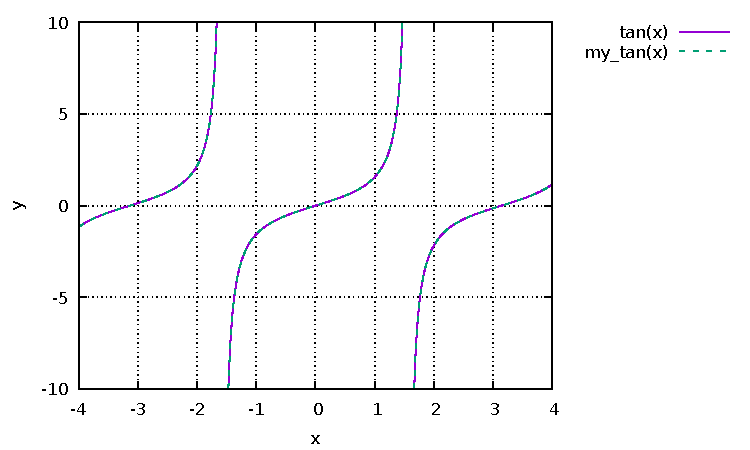
\includegraphics[width=\textwidth]{plot.pdf}
\caption{The tangent function \texttt{tan} from \texttt{<math.h>} compared with the ODE solved \texttt{my\_tan}. 
The difference between the two functions is very small.}
\label{fig:tan}
\end{figure*}

\end{document}
